\documentclass[]{article}

%opening
\title{Vision and Perception}
\author{Nijat Mursali}
\usepackage{tikz}
\usetikzlibrary{calc,intersections,through,backgrounds}
\usepackage{graphicx}
\begin{document}

\maketitle

\begin{abstract}
	This document is used to illustrate all the homework exercises that has been given during Vision and Perception course in 2020/21. There are overall 10 exercises that needed to be done during this time. 


\end{abstract}

\section{Homework 1 - Degenerate Conic}
As mentioned during the video of Geometric Parameters, we needed to compute the $M_{2}$ as we did for $M_{1}$ and then computing the null space of $M_{1}$ and verifying that is 2, then computing the cross product of null space vectors and after normalizing to obtain the $x_{3} = 1$, we needed to think about the result.
\vspace{0.4em}

The idea is here space of $M_{1}$ and verifying that is 2, then computing the cross product of null space vectors and after normalizing to obtain the $x_{3} = 1$, we needed to think about the result.	

\begin{tikzpicture}
\draw (-1.5, 0) coordinate(A) -- (2,0.2) coordinate (B) node [black, scale=1] {$l_{1}$};
\draw (-1,-1) coordinate(C) -- (1.5,1.5) coordinate (D) node [black, scale=1] {$l_{2}$};
\node[red,scale=3] at (intersection of  A--B and C--D){.};
\end{tikzpicture}

Thus, we need to consider the two intersecting lines that we have seen in our lecture: 

\centerline {
$l_{1} = (0.2500, 3.200, 1.0000)^T$  
$l_{2} = (-2.0000, 0.5000, 1.0000)^T$ 
}

\centerline {
	$x = l_{1}xl_{2} = (-0.4138, 0.3448, 1.0000)^T$
}

\vspace{0.5em}

\centerline {
$M_{1} = l_{1}l_{1}^T = 
\left( {\begin{array}{*{20}c}
	0.0625 & 0.8000 & 0.2500 \\
	0.8000 & 10.2400 & 3.2000 \\
	0.2500 &  3.2000 & 1.0000   
	\end{array} } \right)$
}

Thus, by computing the degenerate conic for $l_{2}$, we could get something following:

\centerline {
$M_{2} = l_{2}l_{2}^T = 
\left( {\begin{array}{*{20}c}
	4.0000 & -1.0000 & -2.0000 \\
	-1.0000 & 0.2500 & 0.5000 \\
	-2.0000 &  0.5000 & 1.0000   
	\end{array} } \right)$
}

As we see from the book, the null space can be computed by span as following:

\centerline {
	$Null(M_{1}) = Span\{\left( {\begin{array}{*{20}c}
	0.2210 \\
	0.2751 \\
	-0.9357  
	\end{array} } \right),\left( {\begin{array}{*{20}c}
	-0.9724 \\
	 0.1353 \\
	-0.1899  
	\end{array} } \right) \}$ 
}

and 

\centerline { $Null(M_{2}) = Span\{\left( {\begin{array}{*{20}c}
	0 \\
	0.8944 \\
	-0.4472  
	\end{array} } \right),\left( {\begin{array}{*{20}c}
	-0.4880 \\
	-0.3904 \\
	-0.7807  
	\end{array} } \right) \}$ }

Finally, we need to calculate the cross-product of the null-space components of $M_{1}$ as:

$M_{1} = (0.2210, 0.2751, -0.9357)x(-0.9724, 0.1353, -0.18,99) = (0.0744, 0.9518, 0.2974)^T$
\vspace{0.2em}
then, for $M_{2}$ it will be like:
\vspace{0.2em}

$M_{2} = (0, 0.8944 - 0.4472) x (-0.4880, -0.3904, -0.7807) = (-.8728, 0.2182, 0.4365)^T$

We come up to the result that these two results are no more than the original lines, $l_{1}$ and $l_{2}$ with unitary norm.  

\section{Homework 2 - Five Points Define a Conic}
For each point the conic passes through 

\centerline {$ax_{i}^2 + bx_{i}y_{i} + cy_{i}^2 + dx_{i} + ey_{i} + f = 0$ }
\vspace{0.4em}

thus to determine the parameters of the equation, we need at least five points. Consider the following: 

\centerline {
	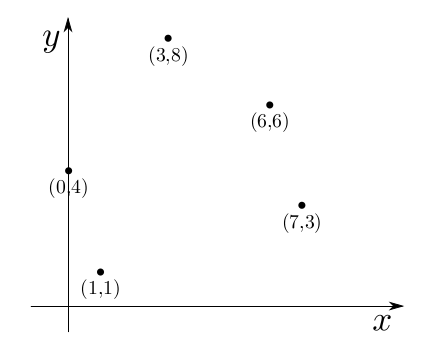
\includegraphics[scale=0.5]{scr2}
}

As we see from the equation, we need to determine the parameters of the equation with at least five points. So, for this homework we just chose 4 points in xy plane with different values, thus we have the following set of equations:

\centerline {
	$\left[ {\begin{array}{*{20}c}
			0 & 0 & 16 & 0 & 4 & 1 \\
			1 & 1 & 1  & 1 & 1 & 1 \\
			9 & 24 & 64  & 3 & 8 & 1 \\
			36 & 36 & 36  & 6 & 6 & 1 \\
			49 & 21 & 9  & 7 & 3 & 1\\   
	\end{array} } \right] 
	\left[ {\begin{array}{*{20}c}
			a \\ 
			b \\ 
			c \\ 
			d \\ 
			e \\ 
			f    
	\end{array} } \right] = 0 $
}

from which we obtain the following values:

\centerline {
	$a = 0.0876$, $b = 0.0258$, $c = 0.0532$, $d = -0.7038$, $e = -0.4629$, $f = 1$,  
}

thus giving us following result:

\centerline {
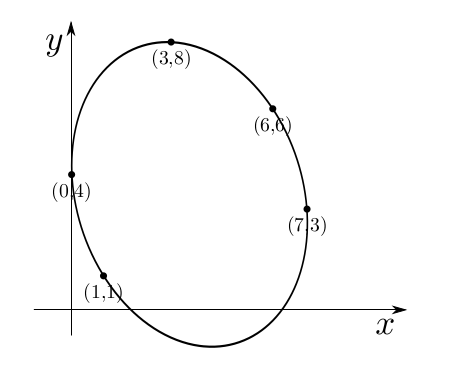
\includegraphics[scale=0.5]{scr1}
}


\section{Homework 3 - Compute the DLT algorithm}
In order to solve this problem, we needed to take one picture and apply the algorithm to check the coordinates of the shape. The idea is to pick 4 points on two different images by hand and apply the DLT algorithm showing the calculations. Additionally, the point selection is arbitrary. 

Thus, we consider the following picture:

\centerline {
	
\includegraphics[scale=0.4]{src}
}

The fundamental goal of ours is to apply homography so that the outline shape of object forms a rectangle. The homogeneous coordinates for the shape are:

\centerline {
	$A = \left[ {\begin{array}{*{20}c}
		281.0 & 234.0 & 1.0 \\
		587.0 & 580.0 & 1.0 \\
		808.0 & 375.0 & 1.0 \\
		506.0 & 45.0 & 1.0
		\end{array} } \right]$
}

and our target shape has the coordinates: 

\centerline {
	$B = \left[ {\begin{array}{*{20}c}
		172.0 & 347.0 & 1.0 \\
		566.0 & 580.0 & 1.0 \\
		763.0 & 340.0 & 1.0 \\
		336.0 & 166.0 & 1.0
		\end{array} } \right]$
}

thus yielding the following equation: 

\centerline {
	$B = AH$
}


in which we ought to find the homography that produces such transformation. The matrix A is non-square, thus it cannot be inverted, we have to resort to the Direct Linear Transformation algorithm, in which at least three non-co-linear points are used to find the 8 independent terms of the transformation matrix. Since our settings have four points, our system is over determined, from which we derive the following transformation matrix:

\vspace{0.5em}

\centerline {
	$H = \left[ {\begin{array}{*{20}c}
		9.7955 & 2.1074 & -1.4142 \\
		-3.4637 & 7.1861 & 2.9439 \\
		-4.2166 & -1.3235 & 1.000
		\end{array} } \right] $
}

\vspace{0.5em}

from which we finally obtain the following transformation:

\vspace{0.5em}
\centerline {
	
\includegraphics[scale=0.4]{out}
}

\vspace{0.5em}

\section{Homework 4 - Affine Transformations}

The task for this exercise is to show that an affine transformation preserves both parallel lines and area. As we have talked in the lecture, we have: 

\centerline {
	$l_1 = (0, 1, 1)^T$ and $l_2=(0,2.67,1)^T$
}

These lines are parallel as they cross-product give us the following:

\centerline {
	$l_1 \times l_2 = (-1.67, 0, 0)^T$
}

Points of the two lines can be obtained as follows:

\centerline {
	$p_1$, $p_2 = Null(l_1)$, 
}

\centerline {
	$p_1=(-0.707, 0.500, -0.500)^T$ and $p_2=(-0.707, -0.500, 0.500)$ 
}

Conversely, 

\centerline {
	$q_1$, $q_2 = Null(l_2)$, 
}

\centerline {
	$q_1=(-0.936, 0.123, -0.328)^T$ and $q_2=(-0.351, -0.328, 0.877)$ 
}

Given the following transformation parameters: $\alpha = 0.7$, $s_1=1.4$, $s_2=0.9$, $t_x=t_y=1.2$, we obtain the following affine transformation matrix:

\centerline {
	$H = \left[ {\begin{array}{*{20}c}
		1.07080 & 0.0618 & 1.2000 \\
		0.9019 & 1.8825 & 1.2000 \\
		0 & 0 & 1.0000
		\end{array} } \right] $
}

Applying the affine transformation onto the lines, we obtain:

\centerline {
	$l_1' = l_1H = (0.902, 1.88, 2.20)$ and $l_2' = l_2H = (2.40, 5.02, 4.20)$ 
}

and so, we verify:

\centerline {
	$l_1' \times l_2'=(-3.14, 1.51, 0)^T$
}

Given the last coordinate in 0, we can ascertain that the lines remain parallel after the transformation.

Given the two triangles formed by an arbitrary collection of lines, $l_1, l_2, l_3$ and $l_4$:


\centerline {
	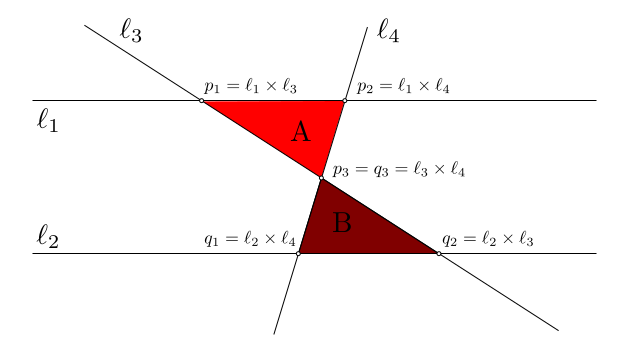
\includegraphics[scale=0.5]{scr4}
}

where $l_1$ and $l_2$ are parallel. We can calculate the area $S$ of the triangles $A$ and $B$, using Heron's relation:

\centerline {
	$S_A = \sqrt{s(s-a)(s-b)(s-c)}$
} 

where s is the semi-perimeter of the triangle $S$.

For triangle A, the relation is as follows:

\centerline {
	$S_A=\sqrt{s_A(s_A - \overline{p_1p_3})(s_A - \overline{p_1p_2}) (s_A - \overline{p_2p_3})}$
}

As for triangle $B$, we have:

\centerline {
	$S_B=\sqrt{s_B(s_B - \overline{p_1p_3})(s_B - \overline{p_1p_2}) (s_B - \overline{p_2p_3})}$
}

Hence, for both triangles, their respective areas can be simply described by the distance of the intersecting points. Given an arbitrarily affine transformation $H$, that can be described as:



\centerline{ $H = \left[ {\begin{array}{*{20}c}
		A & t \\
		\overrightarrow{0} & 1   
		\end{array} } \right]$ }

Taking a line segment of each triangles, we can get the ratio as:

\centerline {
	$\frac{\overline{p_1p_3}}{\overline{q_2q_3}} = \frac{\sqrt{(l_3 \times l_4 - l_1 \times l_3)(l_3 \times l_4 - l_1 \times l_3)}}{\sqrt{(l_3 \times l_4 - l_2 \times l_3)(l_3 \times l_4 - l_2 \times l_3)}}$
}

If we analyze the ratio's behavior under the transformation H by simply multiplying them with H, we get the following equation: 

\centerline {
	$\frac{\overline{p_1p_3}'}{\overline{q_2q_3}'} = \frac{\overline{p_1p_3}}{\overline{q_2q_3}}$
}

This relation can be naturally extended to any two line segments, thus the ratio between the areas of the triangle are also preserved. 


\section{Homework 5 - Homography keeps lines tangent to conics}
Consider the following line $l$, tanget to the conic $C$ at the point $x$, 

\centerline {
	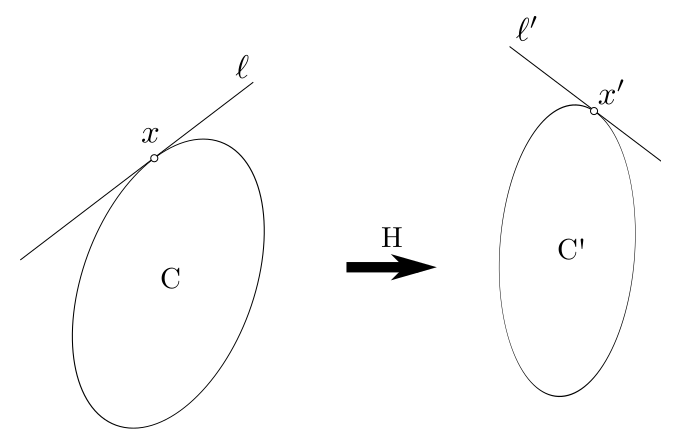
\includegraphics[scale=0.5]{scr3}
}

From this property, we know that $l = Cx$ and $x^Tl=x^TCx = 0$. Using the homography $H$ on $x$, we get $x'=Hx$, and to reverse this transformation, we can use the inverse homography $H^-1$. With the aformentioned properties, we can rewrite the equations like so:

\centerline {
	$x^TCx = (H^-1x')^TC(H^-1x') = 0$
}
this, in turn, is equivalent to :

\centerline {
	$x^TCx = x'(H^-1)^TCH^-1x' = x'C'x' = 0$.
}

From the relation $l = Cx$, we have:

\centerline {
	$(H^-1)^Tl = (H^-1)^TCx$,
}

which can be rewritten to:

\centerline {	
	$(H^-1)^Tl = (H^-1)^TC(H^-1H)x$.
}

As we have previously seen: $C' = (H^-1)^TCH^-1$, and so the previous equation becomes:

\centerline {
	$(H^-1)^Tl = C'Hx$
}

thus finally arriving at:

\centerline {
	$l' = C'x'$
}

which implies that $l'$ is also tangent to $C'$.

\section{Homework 6 - SVD for given matrix}
As we have seen from the example, the matrix A which we out to decompose is the following: 

\centerline{ $A = \left[ {\begin{array}{*{20}c}
		2 & 3 & 1 \\
		1 & 4 & -2   
		\end{array} } \right]$ }
	
The singular value decomposition (SVD) property proposes that any given matrix can be decomposed in three matrices that is:

\centerline { $A = U \Sigma V^T$}

where $\Sigma$ is a rectangular diagonal matrix and, $U$ and $V^T$ are orthogonal matrices. To obtain these matrices, we first compute the product $A^TA$ as following:

\centerline {
	$A^TA = (U \Sigma V^T)^T U \Sigma V^T = V (\Sigma^T \Sigma)V^T $ 
}
which will be equal to 

\centerline{ $A^TA = \left[ {\begin{array}{*{20}c}
		5 & 10 & 0 \\
		10 & 25 & -5 \\ 
		0 & -5 & 5   
		\end{array} } \right]$ }
	
from this relation, we extract the eigenvalues of $A^TA$ as follows:
	
\centerline {
	$(A^TA - I \lambda) x = 0$
}

in which, in order to obtain a non-trivial solution, the following property must hold:

\centerline {
	$det(A^TA - I \lambda) = 0$
}

which gives the following equation:

\centerline {
	$(5- \lambda) (25 - \lambda)(5 - \lambda) - 25(5 - \lambda) - 100(5 - \lambda) = 0 $
}

From this equation, we arrive at the following solutions: 

\centerline {
	$\lambda_{1} = 30$, $\lambda_{2} = 5$, $\lambda_{3} = 0$ 
}

To obtain the eingenvectors, we must find the vectors that lie in the null-space of the resulting matrices once
each eigenvalue is substituted:

For $\lambda = 30$: 

\centerline{ $\left[ {\begin{array}{*{20}c}
		-25 & 10 & 0 \\
		10 & -5 & -5 \\ 
		0 & -5 & -25   
		\end{array} } \right] x = 0$,  }

Giving us the following expressions: 

\centerline {
	$-25x_{1} + 10x_{2} = 0$, 
}
\centerline {
	$10x_{1} - 5x_{2} - 5x_{3} =0$, 
}
\centerline {
	$-5x_{2} - 25x_{3} = 0$	
}

from this linear set of equations, we arrive at the following solution: 

\centerline {
	$x = [-1, -2.5, 0.5]^T$,
}

which is then normalized: 

\centerline {
	$x = [-0.3651, -0.9129, 0.1826]^T$.
}

Repeating the same procedure for the other eigenvalues, we arrive at: 

\centerline {
	$x = [-0.4472, 0, -0.8944]^T$ and $x = [0.8165, -0.4082, -0.4082]^T$
}

Like so, we obtain the matrix $V$, compose of the column vectors: 

\centerline{ $V = \left[ {\begin{array}{*{20}c}
		-0.3651 & -0.4472 & 0.8165 \\
		-0.9129 & 0 & -0.4082 \\ 
		0.1826 & -0.8944 & -0.4082   
		\end{array} } \right]$ 
}
	
furthemore, we also obtain the matrix $\lambda$, which is the square root of the diagonal matrix composed of the calculated eigenvalues: 

\centerline{ $\Sigma = \left[ {\begin{array}{*{20}c}
		\sqrt{30} & 0 & 0 \\
		0 & \sqrt{5} & 0 \\ 
		0 & 0 & 0   
		\end{array} } \right]$ 
}

since the last row is a product of any above row, we can write:

\centerline{ $\Sigma = \left[ {\begin{array}{*{20}c}
		\sqrt{30} & 0 & 0 \\
		0 & \sqrt{5} & 0   
		\end{array} } \right]$ 
}

The last step is to determine the orthonormal matrix $U$. This can be obtained by the following product:

\centerline {
	$AV = U \Sigma V^TV$
} 

where we cross out the $\Sigma V^TV$ that gives us only $AV = U$. Hence:

\centerline{ $\left[ {\begin{array}{*{20}c}
		2 & 3 & 1 \\
		1 & 4 & -2   
		\end{array} } \right] 
			\left[ {\begin{array}{*{20}c}
		-0.3651 & -0.4472 & 0.8165 \\
		-0.9129 & 0 & -0.4082 \\ 
		0.1826 & -0.8944 & -0.4082  
		\end{array} } \right] = U \left[ {\begin{array}{*{20}c}
		\sqrt{30} & 0 & 0 \\
		0 & \sqrt{5} & 0   
		\end{array} } \right]$ 
}

which gives us the following matrix $U$:

\centerline {
	$U = \left[ {\begin{array}{*{20}c}
		-0.6 & -0.8 \\
		-0.8 & 0.6   
		\end{array} } \right]$
}

\section{Homework 7 - Projective Transformation}  
The task here is to find the projective transformation $H$ and define the type of quadric from the quadric equation.

Firstly, let's clarify some points we have learned in our lectures. 

\centerline {
	3D point in $R^3$ which is $X = (X, Y, Z)^T$ in $P^3 : (x_1, x_2, x_3, x_4)^T$,
}

\centerline {
	Euclidean frame $\pi : ax + by + cz +d = 0$, where
	$\pi^TX = 0 => (a b c d) ^T\left[ {\begin{array}{*{20}c}
		x_1 \\
		x_2 \\ 
		x_3 \\
		x_4  
		\end{array} } \right] = 0$	
}

Thus, 

\centerline {
	$X = (X_1, X_2, X_3, X_4)$ derives, 
}
\vspace{0.2em}
\centerline {
		$X^TAX = 4x_1^2 + 4x_1x_2 - 2x_1x_3 + 2x_1x_4 + 5x_2^2 - 2x_2x_4 + 2x_3^2 + 2x_3x_4 + 2x_4^2 = 0$
}

Then, we get the following A matrix,

\centerline {
	$A = a_ia_j = \left[ {\begin{array}{*{20}c}
		4 & 2 & -1 & 1 \\
		2 & 5 & 0 & -1 \\ 
		0 & 0 & 2 &  1 \\
		0 & 0 & 0 & 2  
		\end{array} } \right] = 0 $ 
}

Then from the following equation we are getting the $\lambda$ values. 

\centerline {
	$|\lambda I - A| = \left[ {\begin{array}{*{20}c}
		\lambda - 4 & -2 & 1 & -1 \\
		-2 & \lambda - 5 & 0 & 1 \\ 
		1 & 0 & \lambda - 2 &  -1 \\
		-1 & 1 & -1 & \lambda - 2  
		\end{array} } \right] = 0$
}

\centerline {
	$\lambda ^4 - 13 \lambda ^3 + 52 \lambda ^2 - 81 \lambda + 25 = 0$, 
}

\centerline {
	$\lambda _1 = 6.6637$, $\lambda _2 = 3.6360$, $\lambda _3 = 2.7153$, $\lambda _4 = -0.0151$
}

Then, from the matrix we get the $V$ values, 

\centerline {
	$V_1 = \left[ {\begin{array}{*{20}c}
		-9.2387 \\
		-11.7071 \\ 
		2.1953 \\
		1  
		\end{array} } \right]$, 
	$V_2 = \left[ {\begin{array}{*{20}c}
		0.9476 \\
		-0.6564 \\ 
		0.0319 \\
		1  
		\end{array} } \right]$, 
	$V_3 = \left[ {\begin{array}{*{20}c}
		-0.5125 \\
		0.9964 \\ 
		2.1143 \\
		1  
		\end{array} } \right]$,
	$V_4 = \left[ {\begin{array}{*{20}c}
		-0.6963 \\
		0.4770 \\ 
		-0.8417 \\
		1  
		\end{array} } \right]$,  
}

Then, from the formula of $U_i = AV_i/\sigma _i$, we tried to find the $U$ value and got the following values:

\section{Homework 8 - Point Equations}
The task here is to define the pairs of point equations for the direction and pair of plane equations for coordinate planes. Thus, for a given homogeneous coordinate system in $P^3$, we have the following set of point equations that define the axes:

As we have learned from the lecture 

\centerline {
	$ax_1 + bx_2 + cx_3 + dx_4 = 0$ gives $(a: b: c: d)$
}

where 

\centerline {
	$\pi ^TX = 0$ gives  $(a b c d)^T \left[ {\begin{array}{*{20}c}
		x_1 \\
		x_2 \\ 
		x_3 \\
		x_4   
		\end{array} } \right] = 0$
}

\centerline {
	$x = (1, 0, 0, 1)^T$, $y = (0, 1, 0, 1)^T$ and $z = (0, 0, 1, 1)^T$
} 

and the coordinate planes:

\centerline {
	$x - y = (0, 0, 1, 1)^T$, $y - z = (1, 0, 0, 1)^T$ and $x - z = (0, 1, 0, 1)^T$
}

Given the equation of the quadric used in the previous exercise:

\centerline {
	$X^TAX = 4x_1^2 + 4x_1x_2 - 2x_1x_3 + 2x_1x_4 + 5x_2^2 - 2x_2x_4 + 2x_3^2 + 2x_3x_4 + 2x_4^2$
}

which can be rewritten as: 

\centerline {
	$Q = \left[ {\begin{array}{*{20}c}
		4 & 2 & -1 & 1\\
		2 & 5 & 0 & -1 \\ 
		-1 & 0 & 2 & 1 \\
		1 & -1 & 1 & 2  
		\end{array} } \right]$,
}

as well as the following coordinates of a plane: 

\centerline {
	$\pi = (2, 3, 1, 1)^T$
}

thus giving us the following null space:

\centerline {
	$M_ \pi = \left[ {\begin{array}{*{20}c}
		−0.775 & −0.258 & −0.258 \\
		0.604 & -0.132 & -0.132 \\ 
		-0.132 & 0.956 & -0.044 \\
		-0.132 & -0.044 & 0.956  
		\end{array} } \right]$,
}

From the relation of  $C = M_ \pi ^TQM_ \pi$, we obtain the relation for the conic:

\centerline {
	$C = \left[ {\begin{array}{*{20}c}
		2.617 & 0.717 & −1.437 \\
		0.717 & 2.742 & 1.358 \\ 
		-1.437 & 1.358 & 1.973  
		\end{array} } \right]$,
}

thus, the conic is represented as following:

\centerline {
	$C = 2.617x_1^2 + 0.358x_1x_2 + 2.742x_2^2 - 0.718x_1x_3 + 0.679x_2x_3 + 1.973x_3^2$
}

\section{Homework 9 - Equation of Conic}

As we know from the lecture: 

\centerline {
	$\pi : ax + by + cz + d = 0$ and $n(x,y,z)^T + d = 0$
}

where  $n$ is the normal to the plane computed by $n=(a,b,c)^T$. 

A quadric is a surface in $P3$ defined by the equation 
 
\centerline {
	$X^TQX = 0$
}

where $Q$ is a symmetric $4x4$ matrix. 

The intersection of a plane $\pi$ with a quadric $Q$ is a conic. Computing the conic can be tricky because it requires a coordinate system for the plane. As we know, a coordinate system for the plane can be defined by complement space to $\pi$ as 

\centerline {
	$X= Mx$. 
}

Points on $\pi$ are on $Q$ if 

\centerline {
	$X^TQX = x^TM^TQMx = 0$
}

These points lie on a conic $C$, since $x^TCx = 0$ with $C = M^TQM$.
\section{Homework 10 - Proof for $cos(\alpha)$}  

Points on the plane at infinity $(\pi _ \infty)$, which may be written as $X_ \infty = (d^T, 0)^T$ are mapped to the image plane by a general camera $P = CR[I|t]$ as 

\centerline {
	$x = PX_ \infty = CR[I|t](d^T, 0)^T = CRd$
}

Thus, in this case $H = CR$ is the planar homography between $(\pi _ \infty)$ and the image plane. Since the absolute conic $(\Omega _ \infty)$ is on $(\pi _ \infty)$, we can compute its image as 

\centerline {
	$\omega = (CC^T)^-1 = C^-TC^1$
}
 
Like  $(\Omega _ \infty)$, $\omega$ is an imaginary point conic with no real points. It cannot really be observed in an image. $\omega$ is dependent only on the internal parameters of the camera and is independent of the camera's position or orientation. Thus,
it follows from above that the angle between two rays is given by the simple equation 

The above expression is independent of the choice of the projective coordinate on the image. To see this consider any 2D projective transformation $H$. The points $x_i$ are transformed to $Hx_i$, and $\omega$ transforms to $H^-T \omega H^-1$. Hence, the expression for $cos \omega$ is unchanged. THus it will still be valid for any projective frame. 


\section{Homework 11 - Euclidean Rotation}

The idea here is that dual conic here the duality is between planes and points. Thus, $Q_ \infty ^*$ is made by planes tangent to $(\Omega _ \infty)$, therefore any plane that belongs to $Q_ \infty ^*$ envelope is tangent to $\Omega$. 

\centerline {
	$\pi = \Omega _ \infty X = \pi ^TQ_ \infty ^* = 0$ 
}

\centerline {
	$Q_ \infty ^* = \left[ {\begin{array}{*{20}c}
		I & 0 \\
		0^T & 0   
		\end{array} } \right]$,
}

When we consider the Euclidean transformation represented by the matrix 

\centerline {
	$H_E = \left[ {\begin{array}{*{20}c}
		R & 0 \\
		0^T & 1   
		\end{array} } \right] =  \left[ {\begin{array}{*{20}c}
		cos \theta & -sin \theta & 0 & 0 \\
		sin \theta & cos \theta  & 0 & 0 \\ 
		0 & 0 & 1 & 0 \\ 
		0 & 0 & 0 & 1   
		\end{array} } \right] $,
}

This is a rotation by $ \theta $ about the z-axis with a zero translation. Geometrically it is evident that the family of XY -planes orthogonal to the rotation axis are simply rotated about the Z -axis by this transformation.

This means that there is a pencil of fixed planes orthogonal to the Z -axis. The planes
are fixed as sets, but not point-wise as any (finite) point (not on the axis) is rotated in horizontal circles by this Euclidean action. Algebraically, the fixed planes of H are the eigenvectors of $H^T$.

Corresponding eigenvectors of $H_E^T$ are 

\centerline {
	$E_1 = \left( {\begin{array}{*{20}c}
		1 \\
		i \\ 
		0 \\
		0   
		\end{array} } \right)$, $E_2 = \left( {\begin{array}{*{20}c}
		1 \\
		-i \\ 
		0 \\
		0   
		\end{array} } \right)$, 	$E_3 = \left( {\begin{array}{*{20}c}
		0 \\
		0 \\ 
		1 \\
		0   
		\end{array} } \right)$, 	$E_4 = \left( {\begin{array}{*{20}c}
		0 \\
		0 \\ 
		0 \\
		1   
		\end{array} } \right)$
}

The eigenvectors $E_3$ and $E_4$ are degenerate. Thus there is a pencil of fixed planes which is spanned by these eigenvectors. The axis of this pencil is the line of intersection of the the planes (perpendicular to the Z -axis) with $\pi _ \infty$, and the pencil includes $\pi _ \infty$ .

The example also illustrates the connection between the geometry of the projective
plane, $P_2$ , and projective 3-space, $P_3$ . A plane $\pi$ intersects $\pi _ \infty$ in a line which is the line at infinity,  $l_ \infty$ , of the plane $\pi$. A projective transformation of IP 3 induces a subordinate plane projective transformation on $\pi$.

For defining planes, we have to find the eigenvectors of $H_E^T$ by:

\centerline {
	$[H_E^T - \lambda I]v = 0 $ which gives $\left[ {\begin{array}{*{20}c}
		cos \theta - \lambda & sin \theta & 0 & 0 \\
		-sin \theta & cos \theta - \lambda & 0 & 0 \\ 
		0 & 0 & 1 - \lambda & 0 \\ 
		0 & 0 & 0 & 1 - \lambda   
		\end{array} } \right] $
}

Thus, we have to find such $\lambda$ that satisfies $det(H_E^T - \lambda I) = 0$

\section{Homework 12 - Camera Centre }

The camera centre $C$ is the point for which $PC = 0$. Numerically, this right null-vector may be obtained from the SVD of $R$. Algebraically, the centre $C = (X, Y,Z,T)^T$, where 

\centerline {
	$X=det([p_2, p_3, p_4])$, $Y=-det([p_1, p_3, p_4])$, 
}

\centerline {
	$Z=det([p_1, p_2, p_4])$, $T=-det([p_1, p_2, p_3])$
}

and the $P$ is 

\centerline {
	$P=[M | -MC] = K[R | -RC ]$
}

We can easily find K nad R by decomposing M as $M = KR$ using the $RQ$ decomposition. The matrix $R$ gives the orientation of camera, whereas $K$ is calibration matrix. 

\centerline {
		$K = \left[ {\begin{array}{*{20}c}
		\alpha _x & s & x_0\\
		0 & \alpha _y & y_0 \\ 
		0 & 0 & 1   
		\end{array} } \right]$ and $R|t = \left[ {\begin{array}{*{20}c}
		r_{11} & r_{12} & r_{13} & t_1 \\
		r_{21} & r_{22} & r_{23} & t_2 \\ 
		r_{31} & r_{32} & r_{33} & t_3    
		\end{array} } \right]$
}

For our problem we have $P$ as:

\centerline {
	$P = $
}

Thus, when we decompose the matrix $M$ as $KR$ using QR-decomposition 

\centerline {
	$P = [M| -MC]$ the centre $C = -R^Tt$
}

For our problem, $M$ and $MC$ equals 

\centerline {
	$M = \left[ {\begin{array}{*{20}c}
		0.6773 & 8.6606 & 7.9236 \\
		-4.2765 & 5.4432 & 7.8011 \\ 
		-0.91189 & 0.4426 & 10.4433     
		\end{array} } \right]$, $MC = \left[ {\begin{array}{*{20}c}
		-2000000.61370 \\
		1000 \\ 
		30.0518     
		\end{array} } \right] $
}

Then, we can compute $C$ by



We get  $C$ 

\centerline {
	$C = [\left[ {\begin{array}{*{20}c}
		27964.6 &  19.410.2 & 1635.09   
		\end{array} } \right]^T$
}

b) For this exercise, we needed to find the translation vector which can be calculated as 

\centerline {
	$t = -RC$, thus $t =[\left[ {\begin{array}{*{20}c}
		31751.7 \\
		19688.7 \\ 
		-15127.2   
		\end{array} } \right] $
}


\section{Homework 13 - Calibration Device }
\subsection{Implement a example of a simple calibration device}



\centerline {
	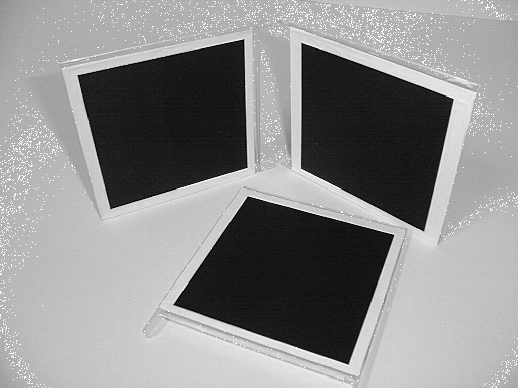
\includegraphics[scale=0.5]{squares}
}

The idea here is to take the image of three squares and compute the K. For this, we need to take several steps. Firstly, we need to find the homography H for each square. 

Then, we need to compute the imaged circular points for the plane of that square as $H(1, \pm i, 0)^T$. 


Before the last step, we need to fit a conic $\omega$ to the six imaged circular points. The constraint that the imaged circular points lie on $\omega$ may be rewritten as two real contrains. If $h_1 \pm ih_2$ lies on $\omega$ then $(h_1 \pm ih_2)^T \omega ()h_1 \pm ih_2) = 0$, and the imaginary and real parts give respectively: 

\centerline {
	$h_1^T \omega h_2 = 0$ and $h_1^T \omega h_1 = h_2^T \omega h_2$
}


which are equations linear in $\omega$. 

Finally, we need to compute the calibration $K$ from $\omega = (KK^T)-1$ using the Cholesky factorization. 

\vspace{0.4em}

Thus, for the first step, we used OpenCV library in order to get the corners of the squares. The points are as following:

\centerline {
		$S_1 =\left[ {\begin{array}{*{20}c}
		77.7704 & 75.5438 & 1.0 \\
		111.0461 & 208.2040 & 1.0  \\ 
		246.7895 & 165.1987 & 1.0 \\
		243.4158 & 38.8666 & 1.0  
		\end{array} } \right] $, $S_2 =\left[ {\begin{array}{*{20}c}
		302.4889 & 42.3844 & 1.0 \\
		301.1318 & 164.1352 & 1.0  \\ 
		423.8295 & 229.9800 & 1.0 \\
		452.5454 & 100.7878 & 1.0  
		\end{array} } \right] $
}

and the last square's coordinates are: 

\centerline {
	$S_3 =\left[ {\begin{array}{*{20}c}
		250.2883 & 197.7703 & 1.0 \\
		174.3199 & 164.1352 & 1.0  \\ 
		423.8295 & 229.9800 & 1.0 \\
		348.1797 & 362.9188 & 1.0  
		\end{array} } \right] $
}

Then, we needed to find the homographies, and we have done it also using the library which gave overall three homographies. 

\vspace{0.5em}

\centerline {
	$H_1 =\left[ {\begin{array}{*{20}c}
		1.09317181e-03 & 4.96735473e-03 & -4.61466910e-01 \\
		4.28243203e-03 & -1.13379462e-03 & -2.42372406e-01  \\ 
		-8.34657587e-04 & -1.04738101e-03 & 1.00000000e+00 
		\end{array} } \right] $
}

\vspace{0.5em}

\centerline {
	$H_2 =\left[ {\begin{array}{*{20}c}
		-4.38946955e-03 & 1.28792782e-02 & 7.44873229e-01 \\
		1.49341334e-02 & -1.30224096e-04 & -4.48894349e+00  \\ 
		3.27712794e-03 & -2.49170706e-03 & 1.00000000e+00
		\end{array} } \right] $
}

\vspace{0.5em}


\centerline {
	$H_3 =\left[ {\begin{array}{*{20}c}
		-4.73274525e-03 & 1.87530587e-02 & -2.50705370e+00 \\
		1.22991572e-02 & 8.54371755e-03 & -4.48894349e+00  \\ 
		2.36397229e-04 & 4.24985472e-03 & 1.00000000e+00
		\end{array} } \right] $
}

Then, we had to find the $\omega$ which we found by A matrix which is found by the columns of $H$ matrix. We have found the $\omega$ as:

\vspace{0.5em}

\centerline {
	$ \omega =\left[ {\begin{array}{*{20}c}
		0.00000000e+00 \\
		7.07106781e-01 \\
		1.11022302e-16 \\
		1.00613962e-16 \\ 
		-7.07106781e-01 \\
		-5.32072216e-16
		\end{array} } \right] $
}

Then, we have divided the $\omega$ with Numpy array into three conics and stored it into the array to find the Cholensky factorization. We have got the new matrix as following:

\vspace{0.5em}

\centerline {
	$ W =\left[ {\begin{array}{*{20}c}
		5.15012402e-01 & 7.07106781e-01 & 1.00613962e-16 \\
		7.07106781e-01 & 1.11022302e-16 & 2.55616781e-01\\
		1.00613962e-16 & 5.42056781e-05 & 3.45077216e-16 
		\end{array} } \right] $
}

\vspace{0.5em}

Finally, using the Cholensky factorization (with \textit{np.linalg}), we have computed the $K$ as following:

\vspace{0.5em}

\centerline {
	$ K =\left[ {\begin{array}{*{20}c}
		1067.7 & -10.4 & 514.3 \\
		0 & 1075.5 & 386.4 \\
		0 & 0 & 1 
		\end{array} } \right] $
}

\vspace{0.5em}


\subsection{Implement Vanishing Points}

Firstly, vanishing point is the image of a point at infinity. Since parallel lines intersect at infinity, the intersection of parallel lines in the image is the vanishing point. As a result, we can two parallel lines, and find the intersection in the image, and the intersection is one vanishing points. Repeat this process, we can find a second and third vanishing point.

As we have discussed in class, there can be several vanishing in an image, depending on where the images were taken. It's also dependent on how many objects you have in the image. In order to find the vanishing points, you need to have several steps in mind: \\

1. remember that all parallel lines will meet in a vanishing point

2. know which lines in the image are really parallel \\ 

For example, in the following picture we have found three vanishing points. 

\vspace{0.5em}

\centerline {
	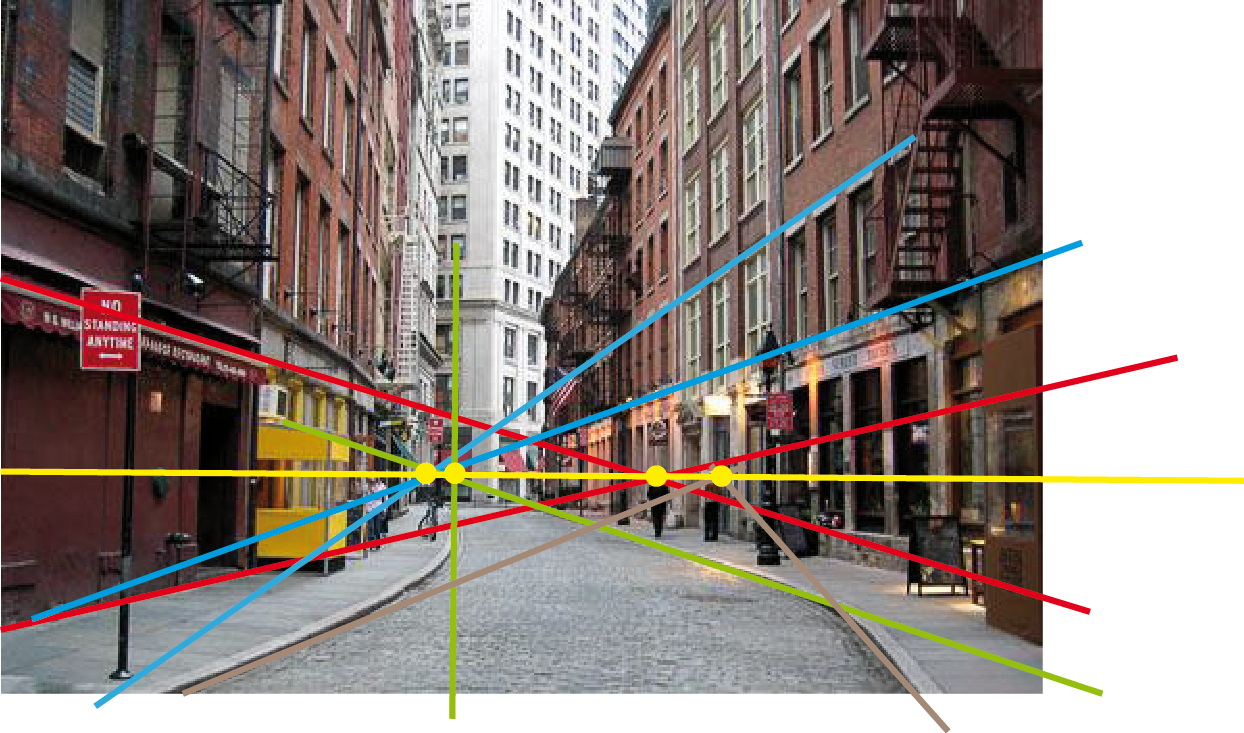
\includegraphics[scale=0.4]{vanishing}
}

\section{Homework 14 - Computing the DLT Algorithm}

The task here was to build a reference shape for calibration as a check-board typically checker-board must not be square. One side must contain an even number of squares and the other side must contain an odd number of squares. We need to measure the dimension of the check-board square. 

Using the harry corner detector, we first found the corners and added them into our code for further computation. At this stage, we get the matrix as following: 

\vspace{0.5em}

\centerline {
	$ x =\left[ {\begin{array}{*{20}c}
		439 & 645 & 219 & 647 & 228 & 24 & 439 & 439 \\
		212 & 410 & 1232 & 606 & 802 & 403 & 1227 & 407 \\
		1 & 1 & 1 & 1 & 1 & 1 & 1 & 1 &  
		\end{array} } \right] $
}

\vspace{0.5em}

When we normalize the matrices (by checking for ratios), we get the following results: 

\vspace{0.5em}

\centerline {
	$ X =\left[ {\begin{array}{*{20}c}
		6 & 9 & 3 & 9 & 3 & 0 & 6 & 6 \\
		3 & 6 & 18 & 9 & 12 & 6 & 18 & 6 \\
		1 & 1 & 1 & 1 & 1 & 1 & 1 & 1 &  
		\end{array} } \right] $
}

\vspace{0.5em}

The next step was to compute the A matrix using the points we have got, but before that we needed to get the correspondences of the coordination points. When, we computed them we also computed the A matrix which had overall 12 columns. 

Then, we have tried to compute $H$ by $H=AA^T$, as our A matrix had 12 columns, when we multiply it with it's transpose it will also give the same columns as $A$. After computing the $H$ matrix, we could get the $V$ by using eigenvectors and after that we could get the $P$ which is the calibration matrix. The following matrix is calibration matrix which is $3 \times 4$:

\vspace{0.5em}

\centerline {
	$ P =\left[ {\begin{array}{*{20}c}
		71.6146 & 0.7109 & -6.2692 & 150.9350 \\
		3.0599 & 67.8655 & -9.5590 & 198.9311 \\
		0.0039 & 0.0017 & -0.0146 & 1.3056   
		\end{array} } \right] $
}

\vspace{0.5em}

As we know from the $Exercise$ $12$, we could find M (which is the first $3 \times 3$ matrix in P) and then we could get the $R$ and $K$ from the QR-decomposition of $M$. The following matrices are $M$, $R$ accordingly. 

\vspace{0.5em}

 \centerline {
 	$ M =\left[ {\begin{array}{*{20}c}
 		71.6146 & 0.7109 & -6.2692  \\
 		3.0599 & 67.8655 & -9.5590  \\
 		0.0039 & 0.0017 & -0.0146    
 		\end{array} } \right] $, $ R =\left[ {\begin{array}{*{20}c}
 		-0.9990 & 0.0426 & -0.00005  \\
 		-0.0426 & -0.9990 & -0.00002  \\
 		-0.00005 & -0.00002 & 0.9999    
 		\end{array} } \right] $
 }

\vspace{0.5em}

Finally, we could find the $K$ which is the following matrix: 

\vspace{0.5em}

\centerline {
	$ K =\left[ {\begin{array}{*{20}c}
		-71.68004 & -3.60745 & 6.67155  \\
		0.00000 & -67.77329 & 9.28266  \\
		0.00000 & 0.00000 & -0.01409    
		\end{array} } \right] $,
}

\vspace{0.5em}

Finally, it was asked to compute the algebraic and geometric errors and then comparing the results obtained by the DLT with the results obtained with the calibration using the absolute conic. In our case error decreased after every iteration and the table is as follows:

\begin{table}[h!]
	\begin{center}
		\label{tab:table1}
		\begin{tabular}{l|c|r} 
			$iter$ & $error$ \\
			\hline
			1 & 1.53 \\
			2 & 1.10 \\
			... & ... \\
			8 & 0.35 \\
		\end{tabular}
	\end{center}
\end{table}


\end{document}
